\subsection{Spezielle Graphen}
\begin{frame}{Vollständige Graphen}
\begin{block}{Vollständiger Graph}
Sei $G = (E, K)$ ein Graph.

$G$ heißt \textbf{vollständig} $:\Leftrightarrow  = E \times E \setminus \Set{e \in E: \Set{e, e}}$
\end{block}

Ein vollständiger Graph mit $n$ Ecken wird als $K_n$ bezeichnet.
\pause
\tikzstyle{vertex}=[draw,fill=black,circle,minimum size=10pt,inner sep=0pt]
\begin{gallery}
    \galleryimage[Green]{vollstaendig/k-1}
    \galleryimage[Green]{vollstaendig/k-2}
    \galleryimage[Green]{vollstaendig/k-3}
    \galleryimage[Green]{vollstaendig/k-4}\\
    \galleryimage[Green]{vollstaendig/k-5}
    \galleryimage[Green]{vollstaendig/k-6}
    \galleryimage[Green]{vollstaendig/k-7}
    \galleryimage[Green]{vollstaendig/k-16}
\end{gallery}
\end{frame}

\begin{frame}{Bipartite Graphen}
\begin{block}{Bipartite Graphen}
Sei $G = (E, K)$ ein Graph und $A, B \subset V$ zwei disjunkte Eckenmengen mit
$E \setminus A = B$.

$G$ heißt \textbf{bipartit} $:\Leftrightarrow \forall_{k = \Set{e_1, e_2} \in K}: (e_1 \in A \text{ und } e_2 \in B) \text{ oder } (e_1 \in B \text{ und } e_2 \in A) $
\end{block}

\begin{gallery}
    \galleryimage[Green]{bipartit/k-2-2}
    \galleryimage[Green]{bipartit/k-2-3}
    \galleryimage[Green]{vollstaendig-bipartit/k-2-5}
    \galleryimage[Green]{vollstaendig-bipartit/k-3-3}\\
    \galleryimage[Green]{vollstaendig-bipartit/k-3-4}
    \galleryimage[Green]{vollstaendig-bipartit/k-3-5}
    \galleryimage[Green]{vollstaendig-bipartit/k-4-5}
    \galleryimage[Green]{vollstaendig-bipartit/k-5-5}
\end{gallery}
\end{frame}

\begin{frame}{Vollständig bipartite Graphen}
\begin{block}{Vollständig bipartite Graphen}
Sei $G = (E, K)$ ein bipartiter Graph und $\Set{A, B}$ bezeichne die Bipartition.

$G$ heißt \textbf{vollständig bipartit} $:\Leftrightarrow \Set{\Set{a, b} | a \in A \land b \in B} = K$
\end{block}

\begin{gallery}
    \galleryimage[red]{bipartit/k-2-2}
    \galleryimage[red]{bipartit/k-2-3}
    \galleryimage[Green]{vollstaendig-bipartit/k-2-5}
    \galleryimage[Green]{vollstaendig-bipartit/k-3-3}\\
    \galleryimage[Green]{vollstaendig-bipartit/k-3-4}
    \galleryimage[Green]{vollstaendig-bipartit/k-3-5}
    \galleryimage[Green]{vollstaendig-bipartit/k-4-5}
    \galleryimage[Green]{vollstaendig-bipartit/k-5-5}
\end{gallery}
\end{frame}

\begin{frame}{Vollständig bipartite Graphen}
Bezeichnung: Vollständig bipartite Graphen mit der Bipartition $\Set{A, B}$ 
bezeichnet man mit $K_{|A|, |B|}$.

\begin{gallery}
    \galleryimage[Green]{vollstaendig-bipartit/k-2-2}
    \galleryimage[Green]{vollstaendig-bipartit/k-2-3}
    \galleryimage[Green]{vollstaendig-bipartit/k-2-5}
    \galleryimage[Green]{vollstaendig-bipartit/k-3-3}\\
    \galleryimage[Green]{vollstaendig-bipartit/k-3-4}
    \galleryimage[Green]{vollstaendig-bipartit/k-3-5}
    \galleryimage[Green]{vollstaendig-bipartit/k-4-5}
    \galleryimage[Green]{vollstaendig-bipartit/k-5-5}
\end{gallery}
\end{frame}

\begin{frame}{Kantenzug}
\begin{block}{Kantenzug}
Sei $G = (E, K)$ ein Graph.

Dann heißt eine Folge $k_1, k_2, \dots, k_s$ von Kanten, zu denen es Ecken
$e_0, e_1, e_2, \dots, e_s$ gibt, so dass
\begin{itemize}
    \item $k_1 = \Set{e_0, e_1}$
    \item $k_2 = \Set{e_1, e_2}$
    \item \dots
    \item $k_s = \Set{e_{s-1}, e_s}$
\end{itemize}
gilt ein \textbf{Kantenzug}, der \textcolor{purple}{$e_0$} und \textcolor{blue}{$e_s$} \textbf{verbindet} und $s$ 
seine \textbf{Länge}.
\end{block}

\adjustbox{max size={\textwidth}{0.2\textheight}}{
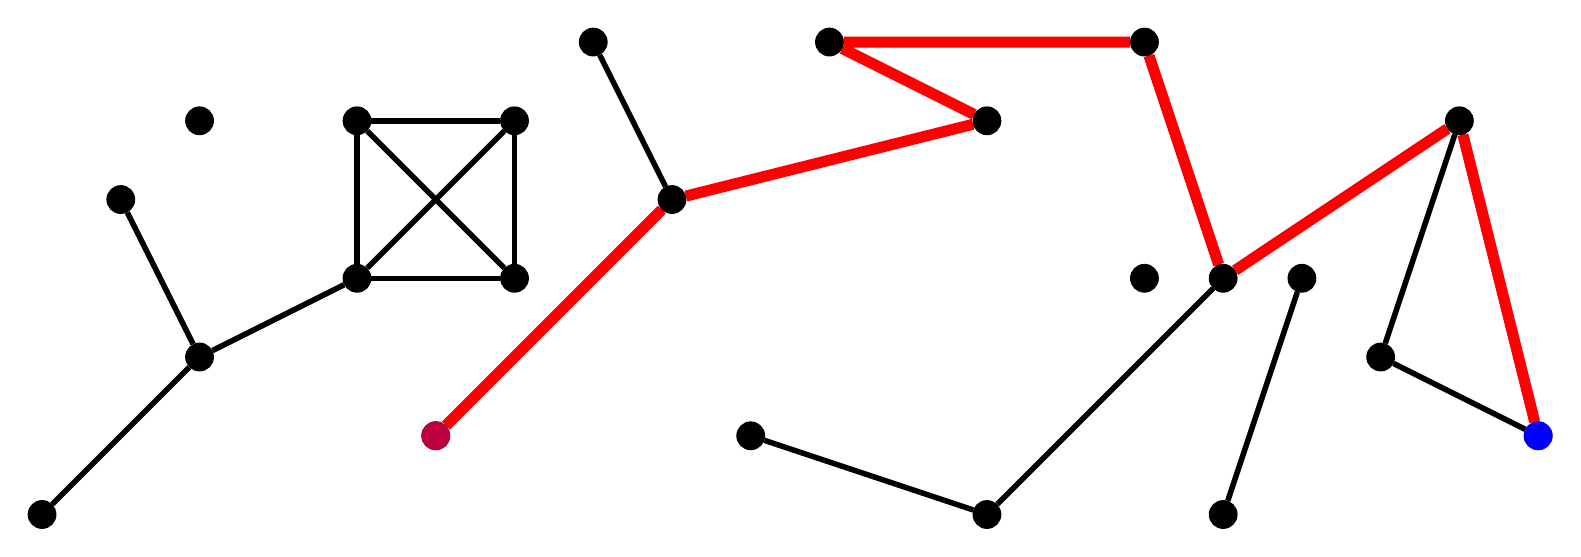
\begin{tikzpicture}
  \node (a)[vertex] at (1,1) {};
  \node (b)[vertex] at (2,5) {};
  \node (c)[vertex] at (3,3) {};
  \node (d)[vertex] at (5,4) {};
  \node (e)[vertex] at (3,6) {};
  \node (f)[vertex] at (5,6) {};
  \node (g)[vertex] at (7,6) {};
  \node (h)[vertex] at (7,4) {};
  \node (i)[vertex] at (6,2) {};
  \node (j)[vertex] at (8,7) {};
  \node (k)[vertex] at (9,5) {};
  \node (l)[vertex] at (13,6) {};
  \node (m)[vertex] at (11,7) {};
  \node (n)[vertex] at (15,7) {};
  \node (o)[vertex] at (16,4) {};
  \node (p)[vertex] at (10,2) {};
  \node (q)[vertex] at (13,1) {};
  \node (r)[vertex] at (16,1) {};
  \node (s)[vertex] at (17,4) {};
  \node (t)[vertex] at (19,6) {};
  \node (u)[vertex] at (18,3) {};
  \node (v)[vertex] at (20,2) {};
  \node (w)[vertex] at (15,4) {};

  \foreach \from/\to in {a/c,c/b,c/d,d/f,f/g,g/h,h/d,d/g,h/f,i/k,k/j,k/l,l/m,m/n,n/o,o/t,t/v,v/u,s/r,o/q,q/p,u/t}
    \draw[line width=2pt] (\from) -- (\to);

  \node (i)[vertex,purple] at (6,2) {};
  \node (v)[vertex,blue] at (20,2) {};
    \draw[line width=4pt, red] (i) -- (k) -- (l) -- (m) -- (n) -- (o) -- (t) -- (v);
\end{tikzpicture}
}
\end{frame}

\begin{frame}{Geschlossener Kantenzug}
\begin{block}{Geschlossener Kantenzug}
Sei $G = (E, K)$ ein Graph und $A = (e_0, e_1, \dots, e_s)$ ein Kantenzug.

A heißt \textbf{geschlossen} $:\Leftrightarrow e_s = e_0$ .
\end{block}

\begin{gallery}
    \galleryimage{walks/walk-1}
    \galleryimage{walks/walk-2}
    \galleryimage{walks/k-3-3-walk}
    \galleryimage{walks/k-5-walk}\\
    \galleryimage{walks/k-16-walk}
    \galleryimage{walks/star-graph-walk}
    \galleryimage{walks/tree-walk}
    \galleryimage{walks/walk-6}
\end{gallery}
\end{frame}

\begin{frame}{Weg}
\begin{block}{Weg}
Sei $G = (E, K)$ ein Graph und $A = (k_1, k_2 \dots, k_s)$ ein Kantenzug.

A heißt \textbf{Weg} $:\Leftrightarrow \forall_{i, j \in 1, \dots, s}: i \neq j \Rightarrow k_i \neq k_j$ .
\end{block}

\pause

\begin{exampleblock}{Salopp}
Ein Kantenzug, bei dem man keine Kante mehrfach abläuft, ist ein Weg.
\end{exampleblock}

\pause

Achtung: Knoten dürfen mehrfach abgelaufen werden!
\end{frame}

\begin{frame}{Kreis}
\begin{block}{Kreis}
Sei $G = (E, K)$ ein Graph und $A = (k_1, k_2 \dots, k_s)$ ein Kantenzug.

A heißt \textbf{Kreis} $:\Leftrightarrow A$ ist geschlossen und ein Weg.
\end{block}

\pause

Manchmal wird das auch "`einfacher Kreis"' genannt.

\pause

\begin{gallery}
    \galleryimage[Green]{graphs/circle-one-facet}
    \galleryimage[Green]{graphs/circle-two-facets}
\end{gallery}
\end{frame}

\begin{frame}{Zusammenhängender Graph}
\begin{block}{Zusammenhängender Graph}
Sei $G = (E, K)$ ein Graph.

$G$ heißt \textbf{zusammenhängend} $:\Leftrightarrow \forall e_1, e_2 \in E: $ Es ex. ein Kantenzug, der $e_1$ und $e_2$ verbindet
\end{block}

\begin{gallery}
    \galleryimage[red]{graphs/graph-1}
    \galleryimage[red]{graphs/graph-2}
    \galleryimage[Green]{graphs/k-3-3}
    \galleryimage[Green]{graphs/k-5}\\
    \galleryimage[Green]{graphs/k-16}
    \galleryimage[Green]{graphs/graph-6}
    \galleryimage[Green]{graphs/star-graph}
    \galleryimage[Green]{graphs/tree}
\end{gallery}
\end{frame}

\begin{frame}{Grad einer Ecke}
\begin{block}{Grad einer Ecke}
Der \textbf{Grad} einer Ecke ist die Anzahl der Kanten, die von dieser Ecke
ausgehen.
\end{block}

\begin{block}{Isolierte Ecken}
Hat eine Ecke den Grad 0, so nennt man ihn \textbf{isoliert}.
\end{block}

\begin{gallery}
    \galleryimage{graphs/graph-1}
    \galleryimage{graphs/graph-2}
    \galleryimage{graphs/k-3-3}
    \galleryimage{graphs/k-5}\\
    \galleryimage{graphs/k-16}
    \galleryimage{graphs/graph-6}
    \galleryimage{graphs/star-graph}
    \galleryimage{graphs/tree}
\end{gallery}
\end{frame}
